%
%                       Documento principal main.tex
%                           Plantilla de Libro            
%                             version:  0.1.0
%      
%                               Contacto:
%                 Github:   https://github.com/medicendav
%                 Correo:   davidtorrezreyes@gmail.com   
%
%-------------------------------------------------------------------------
%
%   Copyright 2020 David Torrez Reyes
%   This file is part of BookTemplate.
%
%   BookTemplate is free software: you can redistribute it and/or modify
%   it under the terms of the GNU General Public License as published by
%   the Free Software Foundation, either version 3 of the License, or
%   (at your option) any later version.
%
%   BookTemplate is distributed in the hope that it will be useful,
%   but WITHOUT ANY WARRANTY; without even the implied warranty of
%   MERCHANTABILITY or FITNESS FOR A PARTICULAR PURPOSE.  See the
%   GNU General Public License for more details.
%
%   You should have received a copy of the GNU General Public License
%   along with BookTemplete.  If not, see <https://www.gnu.org/licenses/>.
%
%-------------------------------------------------------------------------
%
%   Organización de la plantilla:
%   
%   main.tex
%   preámbulo.tex
%   Estilos:
%           constantes.tex
%           entornos.tex
%           encabezados.tex
%           colores.tex
%   Estructura:
%           portada.tex
%           agradecimentos.tex
%           prefacio.tex  
%           tablaContenidos.tex
%           bibliografía.tex
%           indice_palabras.tex                 
%   Capítulos:
%           capitulo_01.tex
%           ...
%   Bibliografía:
%           QFT.bib
%           ...
%   Imágenes:
%           portada.pdf
%           Fuentes:
%                   ...
%   Build:
%           archivos_auxiliares
%           ...
%           main.pdf
%
%---------------------------------------------------------------

%Definimos la clase de documento: En este caso book, con los parámetros opcionales
% s el tamaño de letra (10pt), el tamaÑo de papel (letterpaper) y el formato
% de impresión a dos lados.
\documentclass[10pt,letterpaper,twoside]{book}

%Definimos el archivo preámbulo.tex que se encuentra en el directorio Estilos. De
% modo que cargamos todos los paquetes necesarios para la elaboración del documento.
%
%                       Preámbulo del documento
%
%           Contiene todos los paquetes necesarios para la
%                       compilación del documento
%
%-------------------------------------------------------------------------
%
%Copyright 2020 David Torrez Reyes
%This file is part of BookTemplate.
%
%BookTemplate is free software: you can redistribute it and/or modify
%it under the terms of the GNU General Public License as published by
%the Free Software Foundation, either version 3 of the License, or
%(at your option) any later version.
%
%BookTemplate is distributed in the hope that it will be useful,
%but WITHOUT ANY WARRANTY; without even the implied warranty of
%MERCHANTABILITY or FITNESS FOR A PARTICULAR PURPOSE.  See the
%GNU General Public License for more details.
%
%You should have received a copy of the GNU General Public License
%along with BookTemplete.  If not, see <https://www.gnu.org/licenses/>.
%-------------------------------------------------------------------------




%                  Paquetes de idiomas y codificación
%-------------------------------------------------------------------------
% El paquete inputenc modifica la codificación de entrada de LaTeX.
% Permite escribir con acentos, símbolos inusuales, etc. Como parámetro 
% opcional ingresamos la codificación deseada (latin1) ISO 8859-1.  
\usepackage[utf8]{inputenc}


% El paquete babel gestiona el idioma en el cual se desea trabajar, en
% este caso español (spanish)
\usepackage[spanish]{babel}


% El paquete fontenc gestiona la codificación de salida del documento.
% EL parámetro (T1) indica la codificación estándar de LaTeX
\usepackage[T1]{fontenc}




%                  Paquetes de gráficos, tablas
%-------------------------------------------------------------------------
% El entorno multicol, es de gran utilidad en los sitios donde se
% quieren poner dos figuras una al lado de la otra.
\usepackage{multicol}


% El entorno tabularx, sirve para hacer tablas con  párrafos sin tener que
% indicar  el ancho  de cada  columna de párrafo particular.
\usepackage{tabularx}

% Paquete necesario para la adición de figuras.
% Con el comando \graphcspath indicamos el directorio en el cual se encuentran
% las imágenes a utilizar 
\usepackage{graphicx}
\graphicspath{{Imagenes/}}




%                 Paquetes de configuración de paginas 
%-------------------------------------------------------------------------
% Paquete geometry, gestiona los margenes del documento.
\usepackage[top=3cm,bottom=3cm,left=3cm,right=3cm]{geometry}
\usepackage{lipsum}



%                 Paquetes para la gestión de colores 
%-------------------------------------------------------------------------
% EL paquete xcolor, necesario para la creación y uso de colores.
\usepackage{xcolor}




%     Paquetes para la creación de ecuaciones y simbología matemática 
%-------------------------------------------------------------------------
% Paquetes necesarios para introducir simbología matemática, ecuaciones,
% teoremas, etc.
\usepackage{amsmath}
\usepackage{amsfonts}
\usepackage{amssymb}
\usepackage{amsthm}


% Incluimos el archivo entornos, donde definimos entornos o ambientes creados
% por mi, como frases Celebres, observaciones, etc.
%
%                           	Entornos
%
%           Contiene los comandos necesarios crear nuevos ambientes
%        o entornos de trabajo como frases celebres, observaciones, etc
%
%-------------------------------------------------------------------------
%
%Copyright 2020 David Torrez Reyes
%This file is part of BookTemplate.
%
%BookTemplate is free software: you can redistribute it and/or modify
%it under the terms of the GNU General Public License as published by
%the Free Software Foundation, either version 3 of the License, or
%(at your option) any later version.
%
%BookTemplate is distributed in the hope that it will be useful,
%but WITHOUT ANY WARRANTY; without even the implied warranty of
%MERCHANTABILITY or FITNESS FOR A PARTICULAR PURPOSE.  See the
%GNU General Public License for more details.
%
%You should have received a copy of the GNU General Public License
%along with BookTemplete.  If not, see <https://www.gnu.org/licenses/>.
%-------------------------------------------------------------------------


%                       Mis Entornos
%----------------------------------------------------------------------------
% La sintaxis para la definición de entornos nuevos es
%
% \newenvironment{ENTORNO}[ARGUMENTOS]{ANTES}{DESPUÉS}
%
% En ANTES escribiremos el grupo de comandos que hay que ejecutar al iniciar 
% el entorno y, por tanto, los que le darán el formato al mismo, y DESPUÉS, 
% los que se activarán tras el texto. El resto de elementos funciona como antes.
%-----------------------------------------------------------------------------




%                       Frases Celebres
%%%%%%%%%%%%%%%%%%%%%%%%%%%%%%%%%%%%%%%%%%%%%%%%%%%%%%%%%%%%%%%%%%%%%%
%
% Ejemplo de uso:
% 
% \begin{FraseCelebre}
%   \begin{Frase}
%     ...
%   \end{Frase}
%   \begin{Fuente}
%     ...
%   \end{Fuente}
% \end{FraseCelebre}
%''''''''''''''''''''''''''''''''''''''''''''''''''''''''''''''''''''''
%
% Definición del entorno de Frase Celebre
\newenvironment{FraseCelebre}%
  % Entorno para crear una lista personalizada:
  % \begin{list}{Etiqueta}{Declaraciones}
  % Etiqueta: Marca de los items
  % Declaraciones: Definiciones de longitud  
  {\begin{list}{}{%
    % Definimos margen izquierdo de logitud 0.5 el espacio del texto
    \setlength{\leftmargin}{0.5\textwidth}%
    % No hay espacio extra entre párrafos de la lista 
    \setlength{\parsep}{0cm}%
    % Espacio vertical añadido al inicio y final de la lista
    \addtolength{\topsep}{0.5cm}%
    }
  }
  {\unskip \end{list}}
 

% Definición del entorno de Frase
\newenvironment{Frase}%
  % Alineación a la derecha con estilo cursiva y tamaño \small
  {\item \begin{flushright}%
    \small\em}% 
  {\end{flushright}}


% Definición del entorno de Frase
\newenvironment{FraseA}%
  % Alineación a la derecha con estilo cursiva y tamaño \small
  {\item \begin{center}%
    \small\em}% 
  {\end{center}}

% Definición del entorno de Frase 
\newenvironment{Fuente}%
   % Alineación a la derecha y tamaño de letra \small   
{\item \begin{flushright}\small}%
  {\end{flushright}}
%%%%%%%%%%%%%%%%%%%%%%%%%%%%%%%%%%%%%%%%%%%%%%%%%%%%%%%%%%%%%%%%%%%%





%                       Frases Celebres Centradas
%%%%%%%%%%%%%%%%%%%%%%%%%%%%%%%%%%%%%%%%%%%%%%%%%%%%%%%%%%%%%%%%%%%%%%
%
% Ejemplo de uso:
% 
% \begin{FraseCelebreCentrada}
%   \begin{FraseCentrada}
%     ...
%   \end{FraseCentrada}
%   \begin{FuenteCentrada}
%     ...
%   \end{FuenteCentrada}
% \end{FraseCelebreCentrada}
%''''''''''''''''''''''''''''''''''''''''''''''''''''''''''''''''''''''
%

\newenvironment{FraseCelebreCentrada}%
  % Declaraciones: Definiciones de longitud  
  {\begin{list}{}{%
    % Definimos margen izquierdo de logitud 0 el espacio del texto
    \setlength{\leftmargin}{0cm}%
    % No hay espacio extra entre párrafos de la lista 
    \setlength{\parsep}{0.5cm}%
    % Espacio vertical añadido al inicio y final de la lista
    \addtolength{\topsep}{0.5cm}%
    }
  }
  {\unskip \end{list}}
% Definición del entorno de Frase
\newenvironment{FraseCentrada}%
  % Alineación centrada con estilo cursiva y tamaño \small
  {\item \begin{center}%
    \small\em}% 
  {\end{center}}

% Definición del entorno de Frase Centrada
\newenvironment{FuenteCentrada}%
   % Alineación centrada y tamaño de letra \small   
{\item \begin{center}\small}%
  {\end{center}}
%%%%%%%%%%%%%%%%%%%%%%%%%%%%%%%%%%%%%%%%%%%%%%%%%%%%%%%%%%%%%%%%%%%%


% Incluimos el archivo encargado de generar los encabezados
%
%                   Cabeceras y pies de pagina
%       Formato de las cabeceras de las paginas, por ejemplo
%       nombre del capitulo, sección, numero de pagina, etc.
%
%-------------------------------------------------------------------------
%
%Copyright 2020 David Torrez Reyes
%This file is part of BookTemplate.
%
%BookTemplate is free software: you can redistribute it and/or modify
%it under the terms of the GNU General Public License as published by
%the Free Software Foundation, either version 3 of the License, or
%(at your option) any later version.
%
%BookTemplate is distributed in the hope that it will be useful,
%but WITHOUT ANY WARRANTY; without even the implied warranty of
%MERCHANTABILITY or FITNESS FOR A PARTICULAR PURPOSE.  See the
%GNU General Public License for more details.
%
%You should have received a copy of the GNU General Public License
%along with BookTemplete.  If not, see <https://www.gnu.org/licenses/>.
%-------------------------------------------------------------------------


% Paquete que adminstra los cabeceras
\usepackage{fancyhdr}
% Definimos el estilo general de las cabeceras (fancy)
\pagestyle{fancy}
% Quitamos el estilo de encabezado por defecto
\fancyhf{}
% Predefinímos el comando \chaptermark para que solo nos aparezca
% el numero de Capítulo y su nombre
\renewcommand{\chaptermark}[1]{%
\markboth{\textsc{ \thechapter.}\ #1}{}}
% Predefinímos el comando \sectionmark para que solo nos aparezca
% el numero de Sección y su nombre
\renewcommand{\sectionmark}[1]{%
\markright{\thesection{} #1}{}}

%Paginas pares
\fancyhead[RO]{\rightmark}
\fancyhead[LO]{\thepage}

%Paginas impares 
\fancyhead[LE]{ \leftmark}
\fancyhead[RE]{\thepage}



\newcommand{\cabecera}[1]{%
    \fancyhead[RO]{\textsc{#1}}%
    \fancyhead[LE]{\textsc{#1}}%
}

\newcommand{\restauraCabecera}{%
    % Definimos el estilo general de las cabeceras (fancy)
\pagestyle{fancy}
% Quitamos el estilo de encabezado por defecto
\fancyhf{}

%Paginas pares
\fancyhead[RO]{\rightmark}
\fancyhead[LO]{\thepage}

%Paginas impares 
\fancyhead[LE]{ \leftmark}
\fancyhead[RE]{\thepage}
}

\newcommand{\Agradecimentos}{Agradecimientos\markright{Agradecimentos}}


% Estilo de pagina plana
\fancypagestyle{plain}{%
    \fancyhf{}
    \fancyfoot[C]{\thepage}
    \renewcommand{\headrulewidth}{0pt}
    \renewcommand{\footrulewidth}{0pt}
}


\makeatletter
\def\cleardoublepage{\clearpage\if@twoside \ifodd\c@page\else
  \hbox{}
  \thispagestyle{empty}
  \newpage
  \if@twocolumn\hbox{}\newpage\fi\fi\fi}
\makeatother

% Incluimos el archivo constantes.tex, en el cual tenemos definidos nuevos comandos
% que ayudan a simplificar la escritura del código
%
%                           Constantes
%
%           Contiene constantes definidas como nuevos comandos
%                para la rápida escritura del documento
%
%-------------------------------------------------------------------------
%
%Copyright 2020 David Torrez Reyes
%This file is part of BookTemplate.
%
%BookTemplate is free software: you can redistribute it and/or modify
%it under the terms of the GNU General Public License as published by
%the Free Software Foundation, either version 3 of the License, or
%(at your option) any later version.
%
%BookTemplate is distributed in the hope that it will be useful,
%but WITHOUT ANY WARRANTY; without even the implied warranty of
%MERCHANTABILITY or FITNESS FOR A PARTICULAR PURPOSE.  See the
%GNU General Public License for more details.
%
%You should have received a copy of the GNU General Public License
%along with BookTemplete.  If not, see <https://www.gnu.org/licenses/>.
%-------------------------------------------------------------------------


%   Titulo
%----------------------------:
% \titulo ---> \textbf{Notas de teoría cuántica de campos}
\newcommand{\titulo}{Breve introducción de la teoría cuántica de campos}


%   Autor
%----------------------------:
% \titulo ---> \textbf{Notas de teoría cuántica de campos}
\newcommand{\autor}{David Torrez Reyes}

% Agregamos esquema de colores personalizados
%
%                           	Colores
%
%-------------------------------------------------------------------------
%
%Copyright 2020 David Torrez Reyes
%This file is part of BookTemplate.
%
%BookTemplate is free software: you can redistribute it and/or modify
%it under the terms of the GNU General Public License as published by
%the Free Software Foundation, either version 3 of the License, or
%(at your option) any later version.
%
%BookTemplate is distributed in the hope that it will be useful,
%but WITHOUT ANY WARRANTY; without even the implied warranty of
%MERCHANTABILITY or FITNESS FOR A PARTICULAR PURPOSE.  See the
%GNU General Public License for more details.
%
%You should have received a copy of the GNU General Public License
%along with BookTemplete.  If not, see <https://www.gnu.org/licenses/>.
%-------------------------------------------------------------------------
\usepackage{xcolor}

% Redefinimos el comando \definecolor para que todos los colores sean HTML 
\newcommand{\mycolor}[2]{\definecolor{#1}{HTML}{#2}}


%/*Red*/
\mycolor{red}{F44336}

%/*Pink*/
\mycolor{pink}{E91E63}

%/*Purple*/
\mycolor{purple}{9C27B0}

%/*DeepPurple*/
\mycolor{purpleDeep}{673AB7}

%/*Indigo*/
\mycolor{indigo}{3F51B5}

%/*Blue*/
\mycolor{blue}{2196F3}

%/*LightBlue*/
\mycolor{blueLight}{03A9F4}

%/*Cyan*/
\mycolor{cyan}{00BCD4}

%/*Teal*/
\mycolor{teal}{009688}

%/*Green*/
\mycolor{green}{4CAF50}

%/*LightGreen*/
\mycolor{greenLight}{8BC34A}

%/*Lime*/
\mycolor{lime}{CDDC39}

%/*Yellow*/
\mycolor{yellow}{FFEB3B}

%/*Amber*/
\mycolor{amber}{FFC107}

%/*Orange*/
\mycolor{orange}{FF9800}

%/*DeepOrange*/
\mycolor{orangeDeep}{FF5722}

%/*Brown*/
\mycolor{brown}{795548}

%/*Grey*/
\mycolor{grey}{9E9E9E}

%/*BlueGrey*/
\mycolor{bluegGrey}{607D8B}

%/*White/Black*/
\mycolor{white}{FFFFFF}
\mycolor{black}{000000}


%----------------------------------------------------------------------------
%                              Inicio del documento
%----------------------------------------------------------------------------

% Inicio del documento
\begin{document}
% Estructura
    %
%                           	Portada
%
%           Contiene los comandos necesarios para generar la portada
%                			  del documento
%
%-------------------------------------------------------------------------
%
%Copyright 2020 David Torrez Reyes
%This file is part of BookTemplate.
%
%BookTemplate is free software: you can redistribute it and/or modify
%it under the terms of the GNU General Public License as published by
%the Free Software Foundation, either version 3 of the License, or
%(at your option) any later version.
%
%BookTemplate is distributed in the hope that it will be useful,
%but WITHOUT ANY WARRANTY; without even the implied warranty of
%MERCHANTABILITY or FITNESS FOR A PARTICULAR PURPOSE.  See the
%GNU General Public License for more details.
%
%You should have received a copy of the GNU General Public License
%along with BookTemplete.  If not, see <https://www.gnu.org/licenses/>.
%-------------------------------------------------------------------------


%----------------------------------------------
%				Primera portada
%----------------------------------------------

% Estilo de pagina vacío, No genera encabezado
\thispagestyle{empty}

% Creamos el entorno para generar portada
\begin{titlepage}
	\centering
	% Genera una linea de la longitud del texto con grosor de 1.5 pts
	\rule{\textwidth}{1.5pt} 
		% Cambio tamaño de letra grande (\huge) y texto en negritas
		% Llamamos a la constante \titulo
		{\huge\bfseries		\titulo 	\par}
	% Genera una linea de la longitud del texto con grosor de 1.5 pts
	\rule{\textwidth}{1.5pt} \par
	% Dejamos un espacio de 3cm
	\vspace{3cm}
		% Llamamos a la constante \autor y cambiamos el tamaño de letra a (Large)
		{\huge	\autor \par}
	% Deja un espacio de 3cm
	\vspace{3cm}	
		%Incluimos una imagen de portada
		{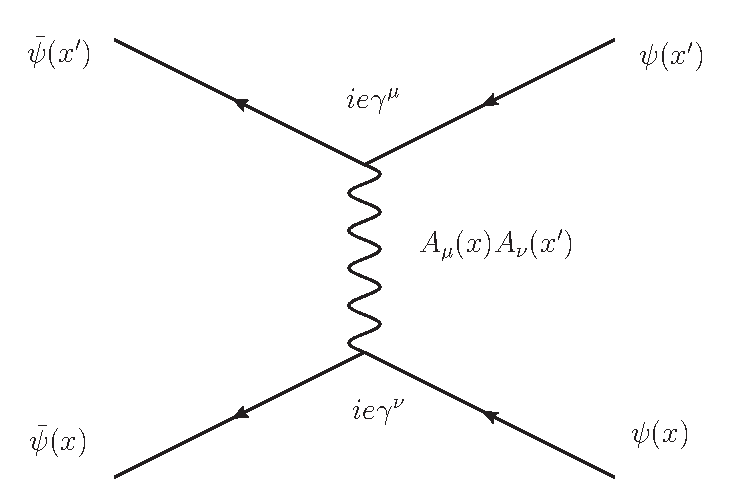
\includegraphics{diagrama_portada} \par}
		% Dejamos un espacio de 2.5cm
	\vspace{2.5cm}
		% Generamos la fecha
		{\huge	\today \par}
		% Genera una linea de la longitud del texto con grosor de 1.5 pts
	\rule{\textwidth}{1.5pt}
\end{titlepage}

%----------------------------------------------
%				Segunda portada
%----------------------------------------------

% Estilo de pagina vacío, No genera encabezado
\thispagestyle{empty}
% Creamos el entorno para generar portada
\begin{titlepage}
	\centering
	\vspace{10cm}
	% Genera una linea de la longitud del texto con grosor de 1.5 pts
	\rule{\textwidth}{1.5pt} 
		% Cambio tamaño de letra grande (\huge) y texto en negritas
		% Llamamos a la constante \titulo
		{\huge\bfseries		\titulo 	\par}
	% Genera una linea de la longitud del texto con grosor de 1.5 pts
	\rule{\textwidth}{1.5pt}
	% Termina el párrafo del titulo
	\par
	% Deja un espacio de 5cm
	\vspace{5cm}	
		{\huge Notas de Teoría Cuántica de Campos \par}
	% Deja un espacio de 5cm
	\vspace{4cm}
	% Llamamos a la constante \autor y cambiamos el tamaño de letra a (Large)
		{\huge	\autor \par}
	% Dejamos un espacio de 3cm
	\vspace{4cm}
		% Generamos la fecha
		{\Large	\today \par}
	\vspace{3cm}
		% Copyright
		{\Large \copyright{} Copyright  2020  \autor}

	\end{titlepage}


    %
%                            Agradecimientos
%
%-------------------------------------------------------------------------
%
%Copyright 2020 David Torrez Reyes
%This file is part of BookTemplate.
%
%BookTemplate is free software: you can redistribute it and/or modify
%it under the terms of the GNU General Public License as published by
%the Free Software Foundation, either version 3 of the License, or
%(at your option) any later version.
%
%BookTemplate is distributed in the hope that it will be useful,
%but WITHOUT ANY WARRANTY; without even the implied warranty of
%MERCHANTABILITY or FITNESS FOR A PARTICULAR PURPOSE.  See the
%GNU General Public License for more details.
%
%You should have received a copy of the GNU General Public License
%along with BookTemplete.  If not, see <https://www.gnu.org/licenses/>.
%-------------------------------------------------------------------------




% Estilo de pagina vacío, No genera encabezado
\thispagestyle{plain}

% Dejando un espacio entre el margen superior y la frase
\vspace*{0.4\textwidth}

% Frase Celebre Centrada.... Ver entornos.tex
\begin{FraseCelebreCentrada}
  \begin{FraseCentrada}
    Nos encontramos en los comienzos mismos de la era de la raza humana.\\
    No es ilógico que tengamos o que tropecemos con problemas, \\
    pero hay decenas de miles de años en el futuro. \\
    Es responsabilidad nuestra hacer lo que podamos, \\
    aprender lo que podamos, mejorar las soluciones y \\
    transmitirlas a nuestros sucesores. \\
    Es responsabilidad nuestra dejar las manos libres a las generaciones futuras
  \end{FraseCentrada}
  \begin{FuenteCentrada}
    Richard P. Feynman
  \end{FuenteCentrada}
\end{FraseCelebreCentrada}

% Nueva pagina
\newpage



\thispagestyle{plain}
\phantomsection
\addcontentsline{toc}{chapter}{Agradecimientos}

\chapter*{Agradecimentos}
\cabecera{Agradecimentos}
\begin{FraseCelebre}
  \begin{Frase}
    Había una vez...
  \end{Frase}
  \begin{Fuente}
    MeDicenDav
  \end{Fuente}
\end{FraseCelebre}


...


\cleardoublepage
\restauraCabecera
    %
%                       Preámbulo del documento
%
%           Contiene todos los paquetes necesarios para la
%                       compilación del documento
%
%-------------------------------------------------------------------------
%
%Copyright 2020 David Torrez Reyes
%This file is part of BookTemplate.
%
%BookTemplate is free software: you can redistribute it and/or modify
%it under the terms of the GNU General Public License as published by
%the Free Software Foundation, either version 3 of the License, or
%(at your option) any later version.
%
%BookTemplate is distributed in the hope that it will be useful,
%but WITHOUT ANY WARRANTY; without even the implied warranty of
%MERCHANTABILITY or FITNESS FOR A PARTICULAR PURPOSE.  See the
%GNU General Public License for more details.
%
%You should have received a copy of the GNU General Public License
%along with BookTemplete.  If not, see <https://www.gnu.org/licenses/>.
%-------------------------------------------------------------------------


\chapter*{Prefacio}
\cabecera{Prefacio}

\begin{FraseCelebre}
    \begin{Frase}
        En ciencia uno intenta decir a la gente,\\
        en una manera en que todos lo puedan entender,\\
        algo que nunca nadie supo antes.\\
        La poesía es exactamente lo contrario.
    \end{Frase}
    \begin{Fuente}
        Paul Adrien Maurice Dirac
    \end{Fuente}
\end{FraseCelebre}


...






\cleardoublepage
\restauraCabecera
    
    %
%                           	Tablas de Contenido
%
%-------------------------------------------------------------------------
%
%Copyright 2020 David Torrez Reyes
%This file is part of BookTemplate.
%
%BookTemplate is free software: you can redistribute it and/or modify
%it under the terms of the GNU General Public License as published by
%the Free Software Foundation, either version 3 of the License, or
%(at your option) any later version.
%
%BookTemplate is distributed in the hope that it will be useful,                 
%but WITHOUT ANY WARRANTY; without even the implied warranty of
%MERCHANTABILITY or FITNESS FOR A PARTICULAR PURPOSE.  See the
%GNU General Public License for more details.
%
%You should have received a copy of the GNU General Public License
%along with BookTemplete.  If not, see <https://www.gnu.org/licenses/>.
%-------------------------------------------------------------------------




% En este archivo se generaran las tablas de contenido como puede ser,
% lista de capítulos, secciones, figuras, ejercicios, etc.  
%                           Configuración
%-------------------------------------------------------------------------

%  Con este comando manejamos el nivel de items de la tabla de contenidos
%  1. Capítulo
%       1.1. Sección
\setcounter{tocdepth}{2}

% Le  pedimos  que nos  numere  todos  los  items hasta  el  nivel
% \subsubsection en el cuerpo del documento.
\setcounter{secnumdepth}{3}

% Creamos los diferentes índices.
% Lo primero un  poco de trabajo en los marcadores  del PDF. No quiero
% que  salga una  entrada  por cada  índice  a nivel  0...  si no  que
% aparezca un marcador "Índices", que  tenga dentro los otros tipos de
% índices.  Total, que creamos el marcador "Índices".
% Antes de  la creación  de los índices,  se añaden los  marcadores de
% nivel 1.

%\ifpdf
%   \pdfbookmark{Índices}{indices}
%\fi



%               Tablas de Contenidos
%....................................................

% No se que haga... Manejar los marcadores del pdf
\ifpdf
   \pdfbookmark[1]{Tabla de contenidos}{tabla de contenidos}
\fi

% Generamos la cabecera del Índice
\cabecera{Índice}
% Creamos la tabla de contenidos
\tableofcontents
% Nueva pagina
\newpage 



%               Índice de Figuras
%....................................................

% No se que haga... Manejar los marcadores del pdf
\ifpdf
   \pdfbookmark[1]{Índice de figuras}{indice de figuras}
\fi

% Creamos el indice de figuras
\listoffigures
% Nueva pagina
\newpage





%               Índice de Tablas
%....................................................

% No se que haga... Manejar los marcadores del pdf
\ifpdf
   \pdfbookmark[1]{Índice de tablas}{indice de tablas}
\fi

% Creamos el indice de figuras
\listoftables
% Nueva pagina
\newpage
\cleardoublepage
\restauraCabecera
\pagenumbering{arabic}

% Capítulos
    %---------------------------------------------------------------------
%
%                          Capítulo 1
%
%---------------------------------------------------------------------

\chapter{Elementos básicos de la mecánica clásica y cuántica}

\begin{FraseCelebre}
\begin{Frase}
    Si consigo ver más lejos es porque\\
    he conseguido auparme a\\
    hombros de gigantes.
\end{Frase}
\begin{Fuente}
    Isaac Newton
\end{Fuente}
\end{FraseCelebre}



%-------------------------------------------------------------------
\section{introducción}
%-------------------------------------------------------------------
\label{cap1:sec:Introduccion}

Toda teoría que desea describir el comportamiento de las partículas elementales se necesita desarrollar bajo  el marco de la teoría cuántica de campos (\textbf{TCC} o en sus siglas en inglés \textbf{TQF}). Aquí se pueden encontrar teorías como la electrodinámica cuántica, el modelo estándar, la teoría de cuerdas, etc.\
La teoría cuántica de campos es el pilar fundamental de nuestra descripción de la Naturaleza. Juega un papel clave en física de la materia condensada,  mecánica estadística y por su puesto en física de altas energías. La teoría cuántica de campos es una potente herramienta matemática que nos permite describir a nuestro universo a distancias $ 10^{-10} \sim 10^{-20} m$, pero la pregunta que emerge de todo esto es ¿Qué es un campo cuántico? y ¿Porqué se necesita un campo cuántico para describir a las partículas que observamos en la naturaleza?\\
De modo que necesitamos una forma de tener una formulación de la mecánica cuántica junto con la relatividad especial, ya que las partículas elementales que conforman a la naturaleza poseen estas características.

%-------------------------------------------------------------------
\section{Convenciones}
%-------------------------------------------------------------------
\label{cap1:sec:Convenciones}

Antes de empezar a profundizar en los cálculos, es necesario definir unas reglas o convenciones como pueden ser las unidades a utilizar. En teorías que describen partículas fundamentales es común utilizar las llamadas \textit{unidades naturales}. 
El uso de este sistema de unidades trae consigo varias ventajas, una de ellas es que simplifican mucho la estructura de las ecuaciones porque elimina las constantes de proporcionalidad y hace que los resultados no dependan del valor de las constantes y se pueda enfocar principalmente en la física del problema.
El sistema mide varias de las magnitudes fundamentales del universo: \textit{tiempo, longitud, masa, carga eléctrica y temperatura}. Se definen haciendo que las cinco constantes de la tabla (\ref{tabla1:Unidades naturales}) tomen el valor la unidad cuando se expresen en ecuaciones y cálculos en dicho sistema.

\begin{table}[h]
\centering    
    \begin{tabular}{| c | c |}
        \hline
        Constante & Símbolo \\
        \hline
        Velocidad de la luz & $c$ \\
        \hline
        Constante de gravitación universal  & $G$ \\
        \hline
        Contante reducida de Plank & $\hbar$ \\
        \hline
        Constante de fuerza de Coulomb & $\frac{1}{4\pi\epsilon_0}$ \\
        \hline
        Constante de Boltzmann & $k$ \\
        \hline
    \end{tabular}
\caption{Unidades naturales.}
\label{tabla1:Unidades naturales}
\end{table}



%-------------------------------------------------------------------
\section{Mecánica clásica}
%-------------------------------------------------------------------
\label{cap2:sec:Mecanica clasica}


Consideremos una partícula puntual de masa $m$ que se mueve en una dimensión bajo la influencia de un potencial independiente del tiempo $V(q)$. De modo que la evolución de la trayectoria de la partícula viene dada por la ecuación de movimiento de Newton, es decir,
\begin{equation*}
    m\ddot{q}=-\frac{dV}{dq}.
\end{equation*}  
Podemos describir este mismo sistema utilizando otro formalismo, encontrando una función $L$ que codifique la evolución del sistema llamada \emph{lagrangiana},
 
\begin{equation*}
    L(q,\dot{q})\equiv T-V=\frac{1}{2}m\ddot{q}^2-V(q),
\end{equation*}
por lo que podemos definir una acción $S$, tal que,
 \begin{equation*}
 S=\int_{\tau_0}^{\tau_1} d\tau L(q(\tau),\dot{q}(\tau)),
 \end{equation*}
 con la cual podemos construir las ecuaciones de movimiento por medio de un principio variacional, es decir el principio de Hamilton, en donde las trayectorias que describen el movimiento real del sistema son aquellas que minimicen la acción. Con lo cual obtenemos la llamada \emph{la ecuación de Euler-Lagrange}.

 \begin{equation*}
    \frac{d}{dt}\frac{\partial L}{\partial \dot{q}}-\frac{\partial L}{\partial q}=0.
\end{equation*} 
  
 Otra formulación equivalente se obtiene definiendo el momento canónico conjugado $p$, definiendo como:
\begin{equation*}
    p=\frac{\partial L}{\partial \dot{q}},
\end{equation*}

usando una transformación de Legendre podemos cambiar del par de variables $(q,\dot{q})$ a las variables $(q,p)$, definiendo una nueva función $H$, llamada Hamiltoniano,
\begin{equation*}
    H(q,p)\equiv p\dot{q}-L(q,\dot{q}).
\end{equation*} 
 De modo que con esta nueva formulación las ecuaciones de movimiento están dadas por las \emph{ecuaciones de Hamilton},

\begin{equation*}   
    \begin{split}        
        \dot{p}&=-\frac{\partial H}{\partial q},\\
        \dot{q}&=\frac{\partial H}{\partial p},
    \end{split}
\end{equation*} 
 
 Por último, tenemos el formalismo de los corchetes de Poisson, donde se definen para dos variables dinámicas cualquiera $A(q,p)$ y $B(q,p)$ que dependan de $q$ y $p$,
\begin{equation*}
    \lbrace A,B \rbrace=\frac{\partial A}{\partial q}\frac{\partial B}{\partial p}-\frac{\partial B}{\partial q}\frac{\partial A}{\partial p}.
\end{equation*}

Veamos que ocurre en el caso de los siguientes corchetes de Poison $\lbrace q,p \rbrace$, $\lbrace q,q \rbrace$ y $\lbrace p,p \rbrace$,

\begin{equation*}
    \begin{split}
        \lbrace q,p \rbrace&=\frac{\partial q}{\partial q}\frac{\partial p}{\partial p}-\frac{\partial p}{\partial q}\frac{\partial q}{\partial p}=1,\\
        \lbrace q,q \rbrace&=\frac{\partial q}{\partial q}\frac{\partial q}{\partial p}-\frac{\partial q}{\partial q}\frac{\partial q}{\partial p}=0,\\
        \lbrace p,p \rbrace&=\frac{\partial p}{\partial q}\frac{\partial p}{\partial p}-\frac{\partial p}{\partial q}\frac{\partial p}{\partial p}=0.\\
    \end{split}
\end{equation*} 

Los cuales son de vital importancia al pasar al formalismo clásico. Por otro lado si queremos encontrar la derivada temporal de la variable dinámica $A(q,p)$, usando las ecuaciones de Hamilton y la definición de los corchetes de Poisson, tenemos,
\begin{equation*}
    \begin{split}
        \frac{dA}{dt}&=\frac{\partial A}{\partial q}\dot{q}+\frac{\partial A}{\partial p}\dot{p}+\frac{\partial A}{\partial t},\\
        &=\frac{\partial A}{\partial q}\frac{\partial H}{\partial p}-\frac{\partial A}{\partial p}\frac{\partial H}{\partial q}+\frac{\partial A}{\partial t},\\
        &=\frac{\partial A}{\partial t}+\lbrace A,H \rbrace.
    \end{split}
\end{equation*} 
 
Los métodos de Lagrange y Hamilton brindan una elegancia y flexibilidad a la hora de describir la dinámica de un sistema.\
Todos estos resultados se pueden generalizar al caso de un número arbitrario $N$ de grados de libertad. De modo que en lugar de tener solo una coordenada $q$ y una $p$, tenemos dos conjuntos de variables dinámicas $q_{i}$ y $p_{i}$ con $i=1,2,...,N$.\

%-------------------------------------------------------------------
\section{Mecánica cuántica}
%-------------------------------------------------------------------
\label{cap3:sec:Mecanica cuantica}

El tratamiento más recurrido para pasar de un formalismo clásico a uno cuántico es la llamada \emph{cuantización de Heisenberg} o primera cuantización; la cual nos dice que tenemos que remplazar las variables dinámicas clásicas del sistema por operadores lineales que actúan sobre un espacio de Hilbert.\
Las variables dinámicas clásicas que se utilizan son $(q,p)\rightarrow(\hat{q},\hat{p})$, operadores cuánticos que no conmutan, es decir, que para cualquiera par de operadores cuánticos $\hat{A}$ y $\hat{B}$se tiene que $[\hat{A},\hat{B}]=\hat{A}\hat{B}-\hat{B}\hat{A}$ que en general es diferente de cero.\\\\
 Este objeto recibe el nombre de \emph{conmutador}, el cual esta relacionado con los corchetes de Poisson de la forma,
 
 \begin{equation*}
 \lbrace A,B \rbrace \rightarrow \frac{1}{i\hbar}[\hat{A},\hat{B}].
 \end{equation*}

Un especial de esta relación ocurre con los operadores $\hat{q},\hat{p}$,

\begin{equation*}
[\hat{A},\hat{B}]=i\hbar
\end{equation*}

Por otro lado sabemos que en la notación de Dirac podemos denotar a cualquier estado de un sistema cuántico por medio del ket $ \ket{\psi} $, además si $ \ket{\psi} $ y $ \ket{\varphi} $ son estados admisibles por el sistema, entonces también lo es su superposición,

\begin{equation*}
\alpha \ket{\psi}+\beta \ket{\varphi}=\ket{\alpha\psi+\beta\varphi}  \hspace{1cm}\forall \alpha,\beta \in \mathbb{C},
\end{equation*} 

Es decir, los estados son elementos de un espacio vectorial complejo, dotado de un producto interno entre los estados $ \ket{\psi} $ y $ \ket{\varphi} $ dado por$ \braket{\varphi}{\psi} \in \mathbb{C} $ que satisface las siguientes propiedades:

\begin{equation*}
    \begin{split}
        &\braket{\varphi}{\psi}=\braket{\psi}{\varphi}^{*}\\
        &\braket{\phi}{\alpha\psi+\beta\varphi}=\alpha\braket{\phi}{\psi}+\beta\braket{\phi}{\varphi},\\
        &\braket{\alpha\psi+\beta\varphi}{\phi}=\alpha^{*}\braket{\psi}{\phi}+\beta^{*}\braket{\varphi}{\phi},\\
        &\braket{\psi}{\psi}\geq 0 \hspace{0.5cm} \forall \ket{\psi},\\
        &\braket{\psi}{\psi}=0 \hspace{0.5cm} \text{solo si} \ket{\psi}=0,
    \end{split}
\end{equation*}

Físicamente podemos interpretar a este producto interno $ \braket{\varphi}{\psi} $ como una amplitud de probabilidad de que el sistema se encuentre en $ \ket{\varphi} $ si esta en el estado $ \ket{\psi} $ solo si los estados están normalizados, es decir $ \braket{\psi}{\psi}=\braket{\varphi}{\varphi}=1 $.

Ademas supondremos que este espacio vectorial complejo equipado con este producto interno es completo y constituye un espacio de Hilbert $\mathcal{H}$.\\

Podemos notar que los  mapeos del tipo $ \braket{\psi}{\cdot}\colon \mathcal{H}\longrightarrow \mathbb{C} $ es decir,  $\ket{\varphi}  \longmapsto \braket{\psi}{\varphi}$ forman también un espacio vectorial donde el vector dual a $ \ket{\psi} $ esta dado por $ \braket{\psi}{\cdot}\equiv\bra{\psi} $ que se conoce como bra.\\

Aterrizando esto a un sistema físico podemos denotar a $ \ket{\textbf{x}} $ como al estado de una partícula localizada en la posición $ \textbf{x} $ y sea $ \ket{\psi} $ su estado general, entonces podríamos formar el "traslape" de estos dos estados $ \braket{\textbf{x}}{\psi} $ que no es otra cosa que la amplitud de probabilidad de que la partícula con estado $ \ket{\psi} $ se encuentre en la posición $ \textbf{x} $ o lo que es lo mismo su función de onda en el espacio de posiciones. De modo que,
\begin{equation*}
\braket{\textbf{x}}{\psi}\equiv \psi(\textbf{x}).  
\end{equation*}  
Por otro lado tenemos que los estados $\{ \ket{\textbf{x}} \arrowvert \hspace{0.1cm} \textbf{x}\in \mathbb{R}^{3} \}$ nos generan una base ortogonal y completa, por lo que cumplen las siguientes propiedades,   

\begin{equation*}
    \begin{split}
	    \braket{ \textbf{x}'}{\textbf{x}}=\delta(\textbf{x}-\textbf{x}'),\\
        \int_{-\infty}^{\infty} d^{3}\textbf{x} \ket{\textbf{x}}\bra{\textbf{x}}=\mathbb{1}.
    \end{split}	
\end{equation*}

De igual manera podemos definir los estados $ \ket{\textbf{p}} $ a través de $ \braket{ \textbf{x}}{\textbf{p}}=e^{i\frac{\textbf{p}\cdot\textbf{x}}{\hbar}} $ nos brinda una nueva base para el mismo espacio de Hilbert, de modo que las relaciones de ortogonalidad y completes son, 

\begin{equation*}
    \begin{split}
        &\braket{ \textbf{p}'}{\textbf{p}}=(2\pi)^{3}\delta(\textbf{p}-\textbf{p}'),\\
        &\int_{-\infty}^{\infty} \frac{d^{3}\textbf{p}}{(2\pi)^{3}} \ket{\textbf{p}}\bra{\textbf{p}}=\mathbb{1}.
    \end{split}
\end{equation*}

Regresando al formalismo de la mecánica cuántica, cada observable físico $A$  esta asociado a un operador lineal  $\hat{A}$ tal que $ \hat{A} \colon \mathcal{H} \longrightarrow \mathcal{H} $, es decir, $ \ket{\psi}\longmapsto  \hat{A} \ket{\psi} =\ket{\text{\^{A}}\psi} $. De modo que obtenemos una ecuación de valores propios $ \text{\^{A}}\ket{\psi_{n}}=\lambda_{n}\ket{\psi_{n}} $ donde $ \lambda_{n} $ son los valores propios del operador \^{A} y $ \ket{\psi_{n}} $ sus vectores propios que constituyen una base ortogonal y completa de modo que podemos usarla para poder obtener el valor esperado del operador \^{A}, esto es,

\begin{equation*}
    \begin{split}
        \expval{\text{\^{A}}}{\psi}&=\bra{\psi}\text{\^{A}} \displaystyle\sum_{n=1} \ket{\psi_{n}}\bra{\psi_{n}}\ket{\psi},\\
        &=\displaystyle\sum_{n=1}\bra{\psi}\text{\^{A}} \ket{\psi_{n}}\bra{\psi_{n}}\ket{\psi},\\
        &=\displaystyle\sum_{n=1}\bra{\psi}\lambda_{n}\ket{\psi_{n}}\bra{\psi_{n}}\ket{\psi},\\
        &=\displaystyle\sum_{n=1}\lambda_{n}\bra{\psi_n}\ket{\psi}^{*}\bra{\psi_{n}}\ket{\psi},\\
        &=\displaystyle\sum_{n=1}\lambda_{n}\lVert\bra{\psi_{n}}\ket{\psi}\rVert^{2},
    \end{split}
\end{equation*}

Por otro lado podemos definir a los traslapes $ \bra{\psi_{n}}{\text{\^{A}}}\ket{\psi_{m}}\equiv A_{nm} $ como los elementos de matriz del operador \^{A} y lo definen por completo.\\\\
Dado un operador cualquiera $\hat{A}$ definimos su \emph{operador hermitico conjugado} $\hat{A}^{\dagger}$ tal que,

\begin{equation*}
    \bra{\varphi}\ket{\hat{A}\psi}=\bra{\hat{A}^{\dagger}\varphi}\ket{\psi} \hspace{0.5cm} \forall \ket{\varphi}, \ket{\psi}  
\end{equation*} 




% Bibliografía e índice alfabético
    %%
%                             Bibliografía
%
%-------------------------------------------------------------------------
%
%   Copyright 2020 David Torrez Reyes
%   This file is part of BookTemplate.
%
%   BookTemplate is free software: you can redistribute it and/or modify
%   it under the terms of the GNU General Public License as published by
%   the Free Software Foundation, either version 3 of the License, or
%   (at your option) any later version.
%
%   BookTemplate is distributed in the hope that it will be useful,
%   but WITHOUT ANY WARRANTY; without even the implied warranty of
%   MERCHANTABILITY or FITNESS FOR A PARTICULAR PURPOSE.  See the
%   GNU General Public License for more details.
%
%   You should have received a copy of the GNU General Public License
%   along with BookTemplete.  If not, see <https://www.gnu.org/licenses/>.
%
%-------------------------------------------------------------------------

\bibliography{Bibliografia/QFT}
% Para que trabajen los hipervínculos
\phantomsection
\addcontentsline{toc}{chapter}{Referencias}
\bibliographystyle{plain}
    %
%                               Indice alfabético
%
%-------------------------------------------------------------------------
%
%Copyright 2020 David Torrez Reyes
%This file is part of BookTemplate.
%
%BookTemplate is free software: you can redistribute it and/or modify
%it under the terms of the GNU General Public License as published by
%the Free Software Foundation, either version 3 of the License, or
%(at your option) any later version.
%
%BookTemplate is distributed in the hope that it will be useful,
%but WITHOUT ANY WARRANTY; without even the implied warranty of
%MERCHANTABILITY or FITNESS FOR A PARTICULAR PURPOSE.  See the
%GNU General Public License for more details.
%
%You should have received a copy of the GNU General Public License
%along with BookTemplete.  If not, see <https://www.gnu.org/licenses/>.
%-------------------------------------------------------------------------

% Para que trabajen los hipervínculos
\phantomsection
% para que lo añada al índice de contenidos
\addcontentsline{toc}{chapter}{Índice alfabético} 
% para que ponga el índice aquí
\printindex 
\end{document}